
\documentclass[12pt,fullpage]{article}

\usepackage{fullpage}
\usepackage{epsfig}
\usepackage{hhline}
\usepackage{enumerate}
\usepackage{enumfrom}
\usepackage{paralist}
\usepackage{amssymb}
\usepackage{multicol}

\input{parsetree.sty}
\newcommand{\npile}[1]{%
  \ptnode{               %
    \( \begin{array}{c}#1%
       \end{array}       %
    \)   }}


\newcommand{\ignore}[1]{}
\newcommand{\nit}[1]{{\it #1}}
\newcommand{\la}{\longleftarrow}

\begin{document}
\thispagestyle{empty}
\pagestyle{empty}

\vspace*{-1.5cm}
\begin{center} \bf
\large  Computational Logic and Automated Reasoning

 Winter  2017~~~ Take Home Examination  \ \ \ \ %Solution Sketches
\end{center}
{\bf Name:} \hspace{7.5cm} {\bf Student Number:}

\vspace{5mm} \noindent
{\bf \large \underline{Instructions}: \ Answer succinctly and clearly.  Explain your answers/solutions.
\ Correct answers without a valid justification count as wrong. Submit by email (to the instructor) a single document in PDF format \underline{prepared with Latex}. \ Include the problem statements with your solutions.} \ Departing from the instructions will make you lose points. \\
\ By default every part of a problem has three points. You get 3 points if the solution is perfect, \ 2 if it is almost perfect, and $0$, otherwise. No points in between.\\
\ {\bf Deadline: April 25 at 23:30.}

\vspace{2mm}\noindent {\bf 1. \ (a)}  \ Assume that you have a finite set of ground facts of the form $R(a,b)$, with arbitrary constants. Assume that they all become the facts for a Prolog program. \ You want to check via Prolog
 if the relation $R$ is symmetric (you do not do anything yourself about checking the property). How would you proceed? Explain if you would add something to the program (and what) and what queries would you pose. Justify. \hfill [3 points]

\noindent {\bf (b)} \ The same as in (b), but about transitivity. \hfill [3 points]\\

\noindent {\bf 2. \ } \ Consider a relational database with the following tables (or set of facts if you want):

\begin{center}
\begin{tabular}{c|c|c|} \hline
$R$ & $A$ & $B$ \\ \hline
& a & b \\
& a & c\\
&c & b\\
&d & e\\
\hhline{~--}
\end{tabular}~~~~~\begin{tabular}{c|c|c|} \hline
$S$ & B & C \\ \hline
& a & b \\
& a & c\\
&c & b\\
&d&a\\
\hhline{~--}
\end{tabular}
\end{center}

\vspace{1mm}This database does not satisfy the sentence $\forall x \forall y(R(x,y) \rightarrow \exists zS(y,z))$. It requires that every value appearing in the second
column in $R$ has to appear in the first column of $S$ accompanied by some value. (In databases this is called a ``referential integrity constraint".)

\vspace{2mm}
\noindent {\bf (a)} \ Define by means of a Prolog program a predicate $V(\cdot,\cdot)$ that collects all the pairs $(x,y)$ from $R$ for which $y$ does not appear in $S$ as indicated above. \hfill [3 points]\\

\noindent {\bf (b)} \ Show how you would use Prolog and predicate $V$ to verify if the integrity constraint is violated. \ Show the execution of Prolog as you understand it, and what you get from it (this is not about running Prolog). \hfill [3 points]\\

\noindent {\bf (c)} \ You  pose to the database above the query in FO predicate logic: \hfill [3 points]
%$$\mathcal{Q}(x)\!: \ \exists y \exists z(R(x,y) \wedge S(y,z) \wedge \forall z (S(y,z) \rightarrow (z = b \vee z=c))).$$
$$\mathcal{Q}(x)\!: \ \exists y \exists z(R(x,y) \wedge S(y,z) \wedge \neg S(z,y)).$$

\newpage \vspace*{-1cm}
Evaluate the query, i.e. find the data values $v$ for variable $x$, such that: \ $D \models \mathcal{Q}[v]$, {\bf by strictly and compositionally applying the inductive definition of formula satisfaction of 
FO predicate logic} (no other method is valid).\\


\noindent {\bf 3. \ } \ Give in detail an explicit   model (i.e. a satisfying structure) for the set of sentences $\Sigma$ below where the extension (contents) of
$\nit{Above}$ {\bf is not} the transitive closure of the extension of $\nit{On}$.

$\Sigma = \{\forall x \forall y (\exists z
(\nit{Above}(x,z) \wedge
\nit{On}(z,y)) \rightarrow \nit{Above}(x,y)), \  \forall x \forall y
(\nit{On}(x,y) \rightarrow
\nit{Above}(x,y))\}$.

\noindent {\bf (a)} \ Verify that the given structure does satisfy $\Sigma$, and \ {\bf (b)} \ Verify the non-transitive closure as explained above. \hfill [3 points each part]. \\

\noindent {\bf 4. \ } \ {\bf (a)} \ Define in first-order predicate logic the symmetric closure of a given binary relation $R(\cdot, \cdot)$. For this introduce a new predicate $S$. \hfill [3 points]\\

\noindent  {\bf (b)} \ Do the same as in (a), but using Prolog. \hfill [3 points]\\

\noindent {\bf 5.} \ You want to use an answer set program (ASP) for 3-Graph-Coloring (3-GC), that you saw in class, to solve a problem about propositional SAT (with formulas in CNF). So, you have to {\em reduce} SAT to 3-GC. \ (This is how you prove that, given that SAT is NP-hard, that 3-GC is also NP-hard. Actually, it is good enough to use the NP-hardness of 3-SAT, about satisfiability of propositional formulas in CNF with each clause having at most  3 literals.) \ The appendix shows how to do the (general) reduction. It takes an instance for 3-SAT, i.e. a formula $\varphi$,  and constructs an instance $G(\varphi)$ for 3-CG, i.e. a graph. It holds: \ $\varphi$ is satisfiable iff $G$ is colorable with 3 colors.\\
\\
{\bf (a)} \ Given the formula $\varphi\!: \ (p \vee \neg r \vee q) \wedge (\neg p \vee r \vee s) \wedge (\neg s \vee p \vee \neg q)$, construct the corresponding graph $G(\varphi)$. \ Explain the correspondence, and draw a picture of the graph. \hfill [3 points]\\
\\
{\bf (b)} \ Write an ASP to solve 3-GC for the resulting graph in (a). \ [2 points] 

Run it with DLV and (clearly explaining) obtain  from it an answer about the colorability of $G(\varphi)$ and the satisfiability of $\varphi$.  Attach \underline{as an appendix} the run with DLV (which implies that the main aspects of the solution should be shown in the main body of the submission). \hfill [5 points]\\

\noindent {\bf (c)} \ Write an ASP that solves the instance of SAT in (a), directly,  without the detour through 3-GC. The methodology should be general, not a hack for this particular instance. So, explain in what sense it is general. \hfill
[3 points]. \\
 
\noindent {\bf (d)} \ Run the program in (c) on DLV, and give the solution to the decision problem accordingly. Also, obtain the answer sets (models) of the program and explain how you interpret them. Attach the run \underline{as an appendix} (which implies that the main aspects of the solution should be shown in the main body of the submission). \hfill [5 points]

%\noindent {\bf 6.} \

\newpage \hspace*{4cm}{\bf \large Appendix: Reducing 3-SAT to 3-GC}

\vspace{0.5cm}

\begin{center}
\begin{figure}[h]
\hspace*{4cm}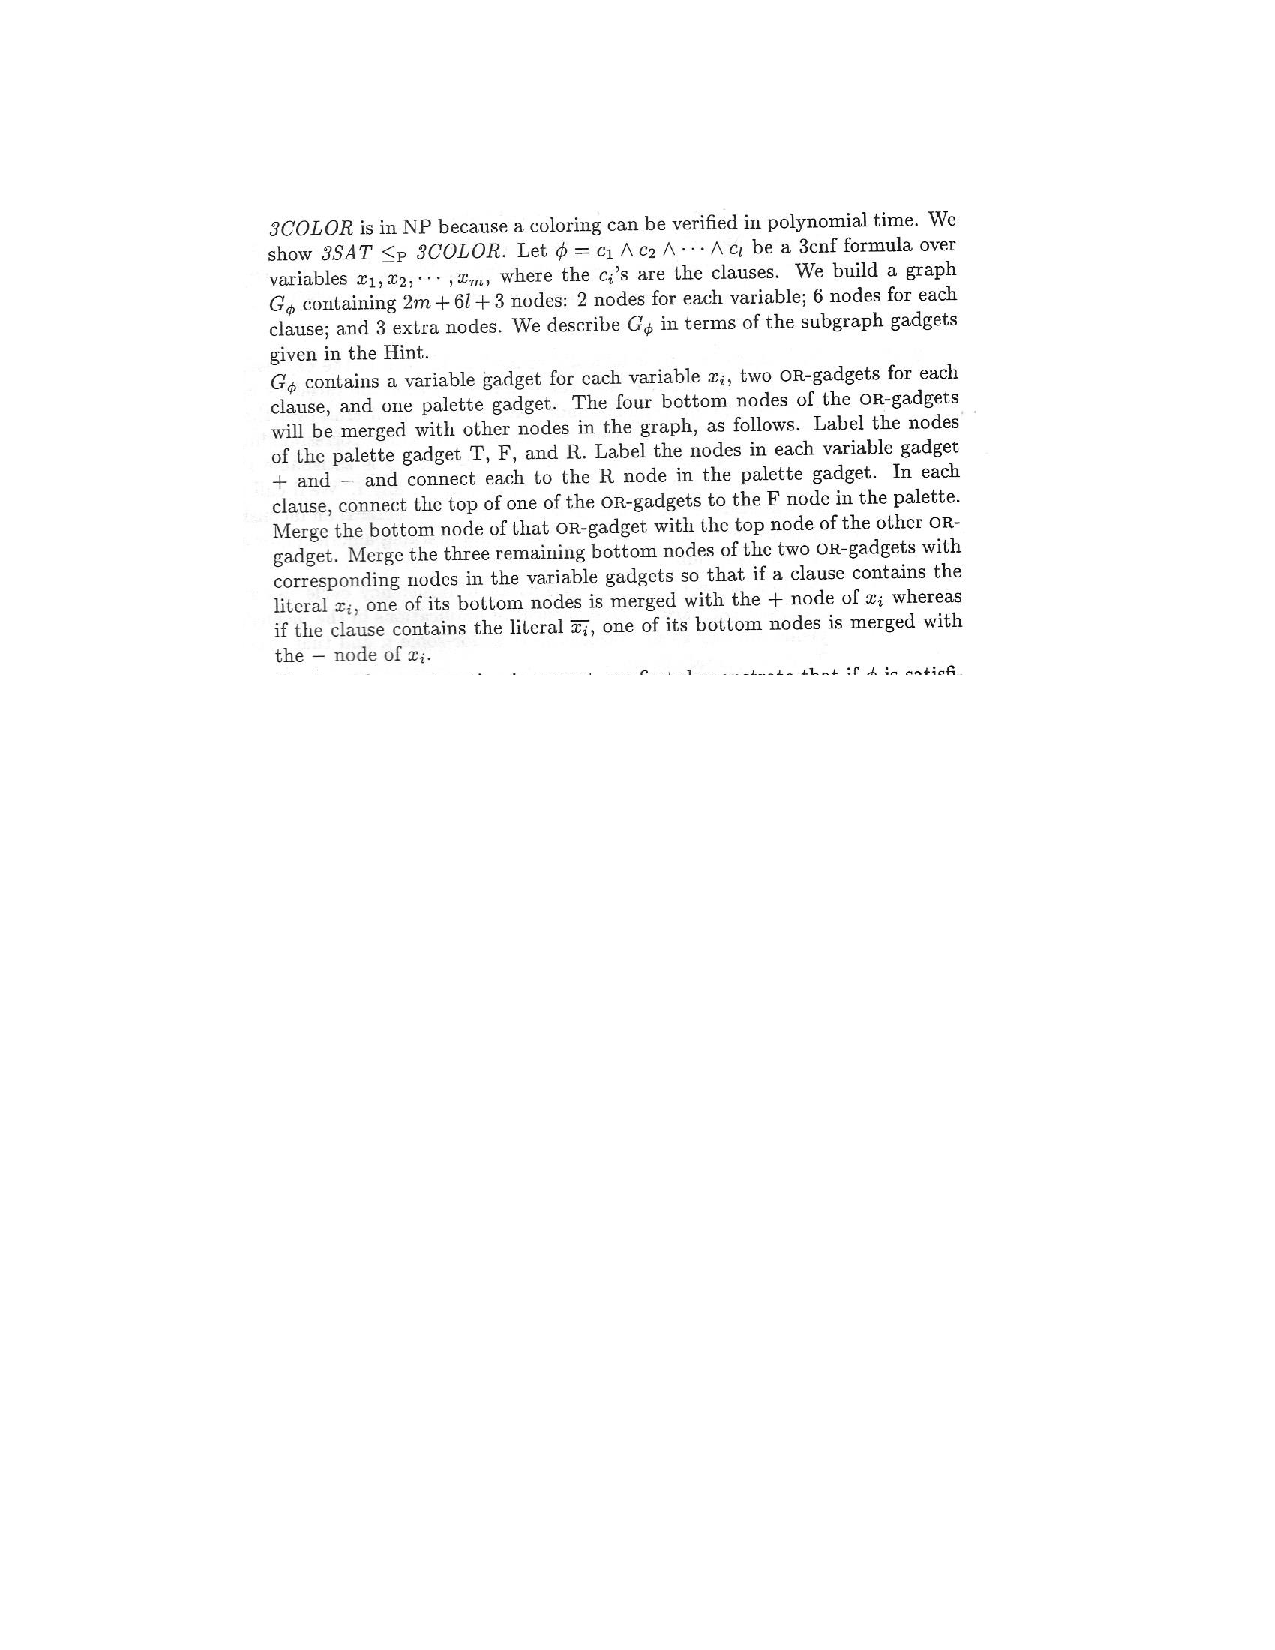
\includegraphics[width=11cm]{proseSAT3Col.pdf}
\end{figure}
\end{center}

\begin{center}
\begin{figure}[h]
\hspace*{4cm}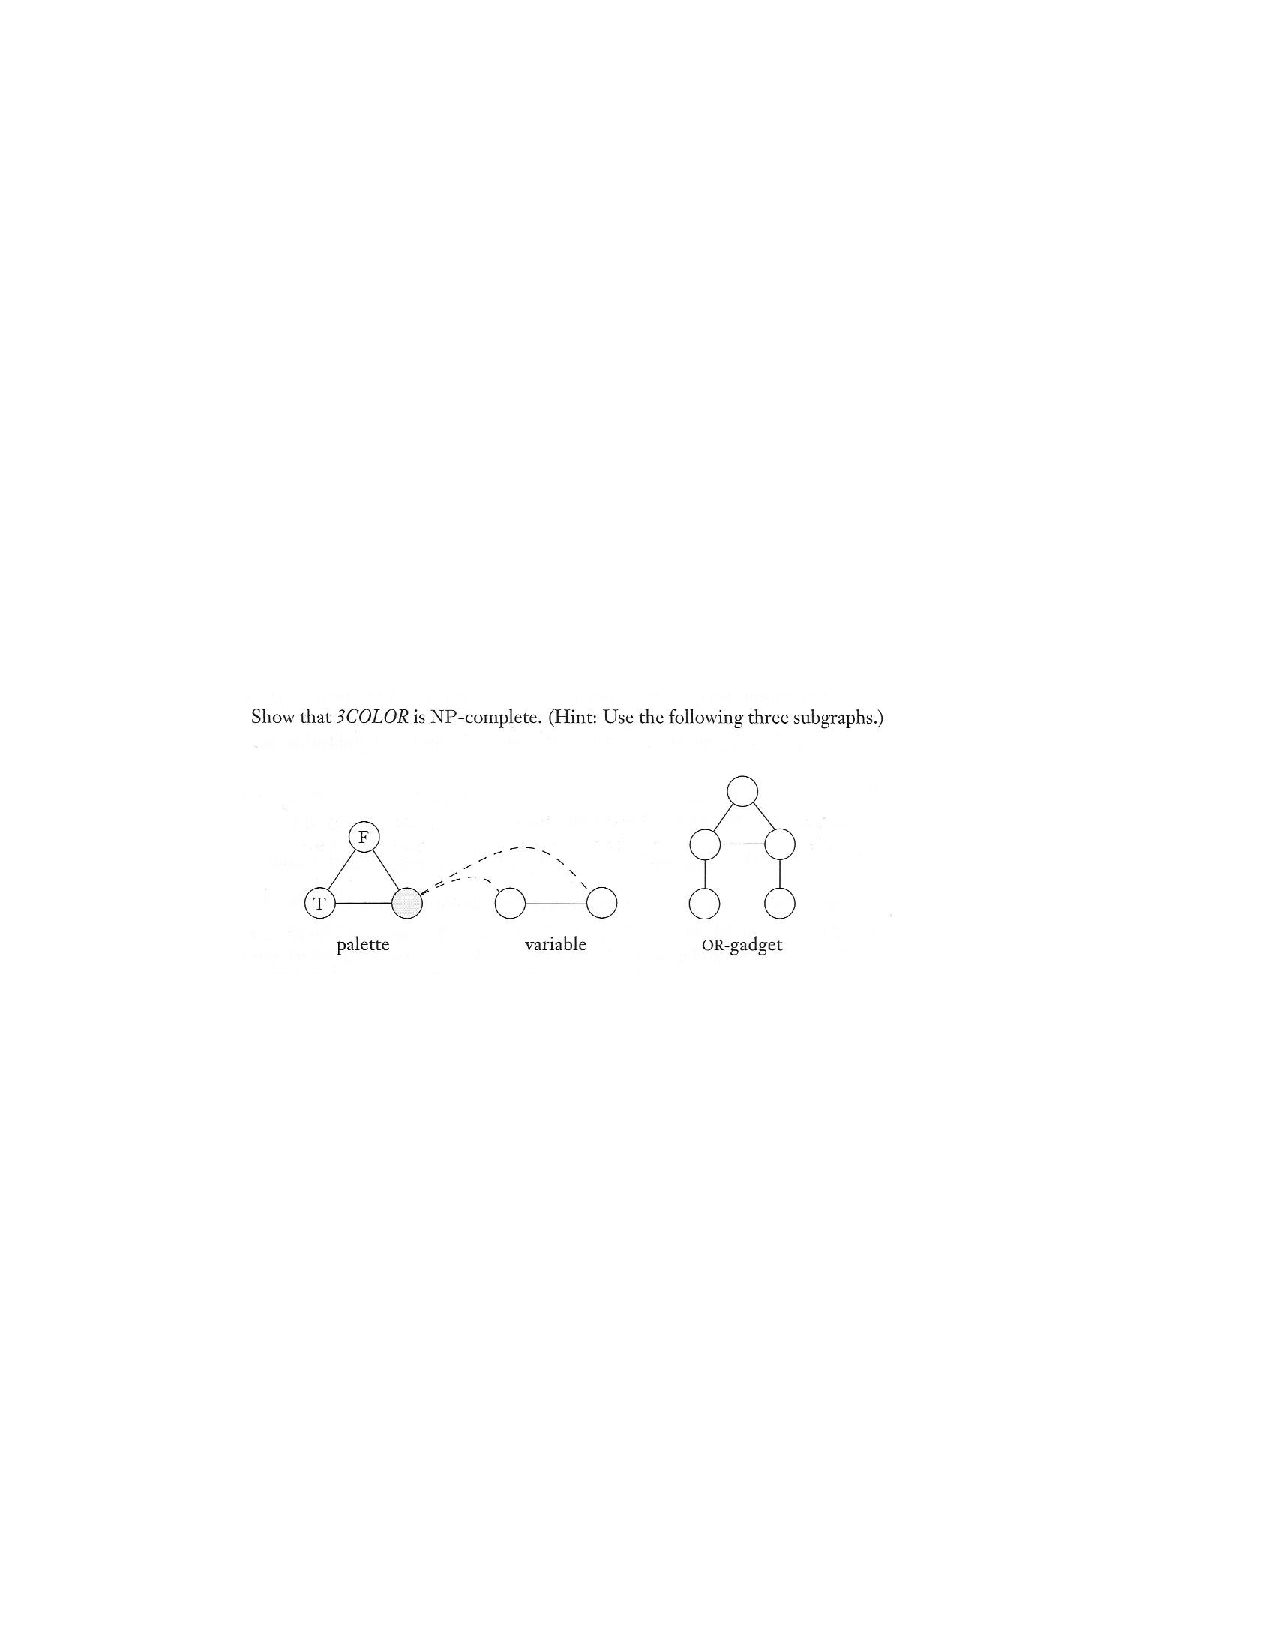
\includegraphics[width=10cm]{figColSAT.pdf}
\end{figure}
\end{center}

\end{document} 